%\localtableofcontents

\vspace{1em}



\section{The history of our Universe and its big open questions}
\label{intro:history_questions}

    Gathering all the knowledge in physics humanity could learn to this day, 
    we are able to come up with a quite interesting and scientifically accurate story,
    describing how our Universe evolved from more than 13.8 billions years ago to nowadays. 
    Our story can explain most of what we observe in the sky, 
    while being consistent with essentially all experimental results obtained on Earth 
    and its Solar neighbourhood.  
    However, the story of our Universe has a few but quite important weak spots. 
    Either because where we do not have 
    a satisfactory physical explanation for some observed phenomena, 
    or simply because some predicted phenomena are not currently observable
    (and potentially will never be).
    That also explain my use of the word \emph{story} instead of \emph{history}, 
    which would only contains verified facts. 

    The story in a nutshell goes as follows: the ``beginning''
    of the Universe\footnote{ The actual beginning of 
    the Universe can be seen as a complex philosophical question or simply as an 
    ill defined physical concept. This discussion is beyond the scope of this work 
    and/or my capabilities. Here, I simply name as ``beginning'' the first epoch of the Universe
    for which we have a widely known physical theory to describe it.}, 
    also known as the \emph{Big Bang} is the start of the \emph{inflation}, 
    an epoch of exponential 
    expansion of space that we believe happened around 13.8 billion years ago. 
    Inflation transformed quantum, microscopic fluctuations of space
    into macroscopic density fluctuations of the Universe's constituents:
    quarks, photons, neutrinos and dark matter. 
    After inflation, the Universe continues to expand but much slowly. 
    The average temperature of the Universe decreases adiabatiacally. 
    Quarks start to gather to form protons, neutrons and relics of heavier atoms, 
    such as deuterium, tritium, helium, lithium and so on. 
    All this during the first few minutes of the Universe's history, in the so called
    \emph{Big Bang nucleosynthesis}. 
    After 380 thousand years, electrons rebind with protons to form neutral 
    hydrogen, while photons scatter for their last time with baryons as the 
    Universe becomes more diffuse. 
    The photons from this epoch are observable today and are known as the 
    \emph{cosmic microwave background}. 
    The Universe then enters its \emph{dark ages}, where hydrogen is mostly neutral and 
    stars have not yet formed. 
    After several million years, gravity clumps hydrogen into dense clouds that reach 
    high enough temperatures to start thermonuclear reactions in their core. 
    The first stars are formed. Then the first galaxies. These galaxies merge into larger 
    galaxies, galaxies form small virialised groups, large groups, clusters, super clusters. 
    Clusters, filamentary structures and voids compose the so called cosmic web. 
    At around half of the Universe's age, the expansion starts to speed up again,
    accelerating, as if gravity became repulsive on very large scales. 
    Then, on one of the many billions of galaxies, the \emph{Milky Way}, 
    planet Earth formed around a somewhat isolated star, the Sun, 
    and here we are today, observing the sky, trying to explain the whole Universe. 

    This story is based on a few assumptions: that general relativity (GR) describes gravity; 
    that the Universe can be modelled as statistically homogeneous and isotropic on large enough
    scales; and that the Universe is composed of the standard model particles and interactions, 
    with the addition of two exotic components: dark energy and dark matter. 

    The origin or nature of the dark sector is one of the biggest mysteries in physics. 
    Several models of dark matter are based on particles beyond the standard model which 
    have not yet been detected, despite the huge experimental efforts towards this goal. 
    The simplest model of dark energy is a cosmological constant which is actually 
    part of GR equations. The possibility that dark energy could be an exotic fluid or 
    the manifestation of an extra force has predicted implications that were not yet 
    observed either. 

    Another weak spot of the story of our Universe is inflation. 
    Up to now, inflation is a successful theory explaining an important set of observations: 
    the homogeneity of the photon temperature 
    from the cosmic microwave background on scales larger than the horizon;
    the flatness of space; and the seeds of structure formation.
    However, the predicted and observable effects of inflation were not yet observed,
    such as primordial gravitational waves.
     
    Solving for the mysteries of the dark sector and inflation 
    would represent major breakthroughs in physics. 
    Large teams of scientists, including myself, are dedicated
    to these puzzles, either theoretically or experimentally. 

    My past work has been focused on observations related to the understanding of dark energy. 
    The rest of this chapter will be dedicated to explaining the problem 
    of accelerated expansion, the dark energy model, alternative solutions,
    and how to observe the expansion. 

\section{Evidences for the accelerated expansion of the Universe}
\label{intro:evidences_acceleration}

    Not long after developing his theory of gravity, Einstein wanted to write a model 
    for a static Universe filled with standard matter. 
    Since gravity is attractive, his solution 
    was to include a new constant term, $\Lambda$, in the equations. 
    This constant, later known as the \emph{cosmological constant}, 
    is one of the simplest models of dark energy, currently
    in agreement with a wide variety of cosmological observations. 
    
    The first indirect evidences for dark energy come from measurements 
    of galaxy clustering in the 1980's 
    (\cite{peeblesTestsCosmologicalModels1984,
    maddoxGalaxyCorrelationsLarge1990, 
    efstathiouCosmologicalConstantCold1990}). 
    At the end of the 1990's, two independent teams measured the expansion of 
    the Universe using type-Ia supernovae as standard candles
    (\cite{riessObservationalEvidenceSupernovae1998, 
    perlmutterMeasurementsOmegaLambda1999}). 
    Their observations could only be explained by 
    an Universe containing around 30 per cent of matter and 70 per cent of dark energy
    in the form of a cosmological constant. 
    Few years later, first measurements of the 
    temperature fluctuations in the cosmic microwave background were consistent with 
    an Universe with a flat space (\cite{balbiConstraintsCosmologicalParameters2000,
    debernardisFlatUniverse2000}), 
    which in combination with measurements of clustering, 
    supernovae and the local expansion rate (\cite{mouldHubbleSpaceTelescope2000}), 
    confirmed the acceleration of our Universe's expansion. 
    Age estimates of globular stellar clusters, which are
    supposed to be among the oldest astrophysical objects, 
    also indicated that the Universe had to be older than the age predicted 
    by models of an Universe only filled with matter (\cite{chaboyerAgeUniverse1998}). 
    The following decade, the 2000's, was enriched with the first measurements
    of the baryon acoustic oscillations in the distribution of galaxies
    (\cite{eisensteinDetectionBaryonAcoustic2005, cole2dFGalaxyRedshift2005}).
    Used as a standard ruler, baryon acoustic oscillations re-confirmed 
    the accelerated nature of the expansion.
    
    Since the 2010's, several cosmological experiments were constructed with the goal of
    improving the precision of all the measurements discussed above. 
    Today, in the 2020's, state-of-the-art measurements of cosmological parameters 
    achieved relative uncertainties of the order of a few percent or less, 
    a quite remarkable score for observational cosmology. 
    Nevertheless, the data shows no evidence for a departure from a model of Universe 
    governed by GR, composed by 70 per cent of this mysterious cosmological 
    constant and 25 per cent by this mysterious dark matter. 

    The future is promising with several stage-IV experiments starting their data taking.
    They will measure millions of galaxy redshifts, billions of galaxy fluxes and shapes, 
    hundreds of thousands of type-Ia supernovae, 
    the cosmic microwave background temperature and polarisation to exquisite 
    precision and resolution, and many more cosmic probes. 
    We truly hope that the data will shed a light over some of the largest mysteries 
    involving our own history. 



\section{Model of an expanding Universe}
\label{intro:model}

    \subsection{Assumptions and ingredients}
    \label{intro:model:ingredients}

    In order to define some important cosmological parameters, I will quickly review
    the basics of the currently most accepted model for our Universe in the limit of 
    very large scales, where it can be considered homogeneous and isotropic. 
    This is also known as the \emph{background} model, since the formation of structures 
    (see next section) can
    be modelled as small perturbations on top of it. 
    It is also assumed that gravity is 
    described by general relativity (GR), which interlinks the fabric of space-time and 
    energy densities of the Universe constituents: 
    \emph{baryons} (protons, electrons, atoms), 
    photons, neutrinos, cold dark matter and dark energy. 

    The expansion of space is usually parametrised by the scale factor $a(t)$, 
    a function of time $t$ that dictates how physical and comoving distances 
    relate to each other. We assume that $a(t_0) = 1$ today ($t_0 = 13.8$ Gyr) 
    and that $a \rightarrow 0$ as $t \rightarrow 0$. The speed of the expansion
    and its acceleration are simply first and second derivatives with 
    respect to time, $\dot{a}(t)$ and $\ddot{a}(t)$, respectively. 
    The expansion rate of the Universe is defined
    as $H(t) = \dot{a}(t)/a(t)$ and takes the Hubble constant value today, 
    $H(t_0) = H_0 = 100 h ~ \mathrm{km/s/Mpc} \sim 70$~km/s/Mpc. 
    Since the scale factor is a monotonically increasing function of time 
    (in our simple model), $a$ is commonly used to describe a given cosmic epoch. 

    One of the consequences of the expansion is that relativistic species, such 
    as photons and massless neutrinos, loose energy or are \emph{redshifted} as they 
    propagate. In astronomy, the redshift $z$ is defined as the relative difference
    in wavelength between the one emitted by source and the one observed.  
    Thus, in an expanding Universe the scale factor is related to the redshift as 
    $a = 1/(1+z)$. Redshift is also commonly used to describe cosmic epoch or distances.
    The time today $t_0$ corresponds to $z=0$ while $z \rightarrow \infty$ as $t \rightarrow 0$. 

    \subsection{The expansion rate}
    \label{intro:model:expansion_rate}

    The expansion rate can be derived from GR equations and be written as a function of 
    redshift and the densities of each constituent
    \begin{equation}
        H^2(z) = H^2_0 \left[ \Omega_m(1+z)^3 + \Omega_r (1+z)^4 + \Omega_{\mathrm{de}}(z) + \Omega_k(1+z)^2\right]
        \label{eq:expansion_rate}
    \end{equation}
    where $\Omega_x = \rho_x / \rho_\mathrm{ crit}$ is the ratio between the density 
    constituent $x$ today and the critical energy density $\rho_\mathrm{ crit} = 3H_0^2/8\pi G$, 
    which is the density required for a flat space geometry. 
    The subscripts $m$, $r$, $de$ and $k$ stand
    for non-relativistic species (baryons, cold dark matter and non-relativistic neutrinos), 
    relativistic species (photons and relativistic neutrinos), dark energy and curvature, 
    respectively. The curvature ``density'' parameter is defined as a function of the others,
    $\Omega_k = (1-\sum_x \Omega_x)$, and it is zero in a flat space geometry.
    Non-relativistic species dilute in an expanding universe so their energy density is 
    proportional to $a^{-3} = (1+z)^3$. Relativistic species dilute as well but have an
    extra factor of $a^{-1}$ due to redshifting. 
    The dark energy term is written as a general function of redshift in Eq.~\ref{eq:expansion_rate}.
    In the simplest case of a cosmological constant, $\Omega_{\mathrm{de}}(z) = \Omega_\Lambda$, i.e. a constant.
    The dependency of curvature with $a^{-2}$ simply comes from the field equations. 

    Figure~\ref{fig:hubble_theory} shows the Hubble expansion rate (times $a(z)$) as a function of redshift $z$
    for a few example of cosmological parameters. All models considered have zero curvature. 
    For all models, the Universe decelerates ($\dot{a}$ decreases) as time goes by (redshift decreases) 
    until dark energy starts to dominate around $z\sim 0.5-0.7$, when the expansion accelerates until today. 
    We can see how the Hubble constant $h$ simply sets the overall amplitude of the curve.
    Also, for increasing values of $\Omega_m$, the transition between matter-dominated to dark energy-dominated era 
    happens at lower redshift. 

    \begin{figure}[t]
        \centering 
        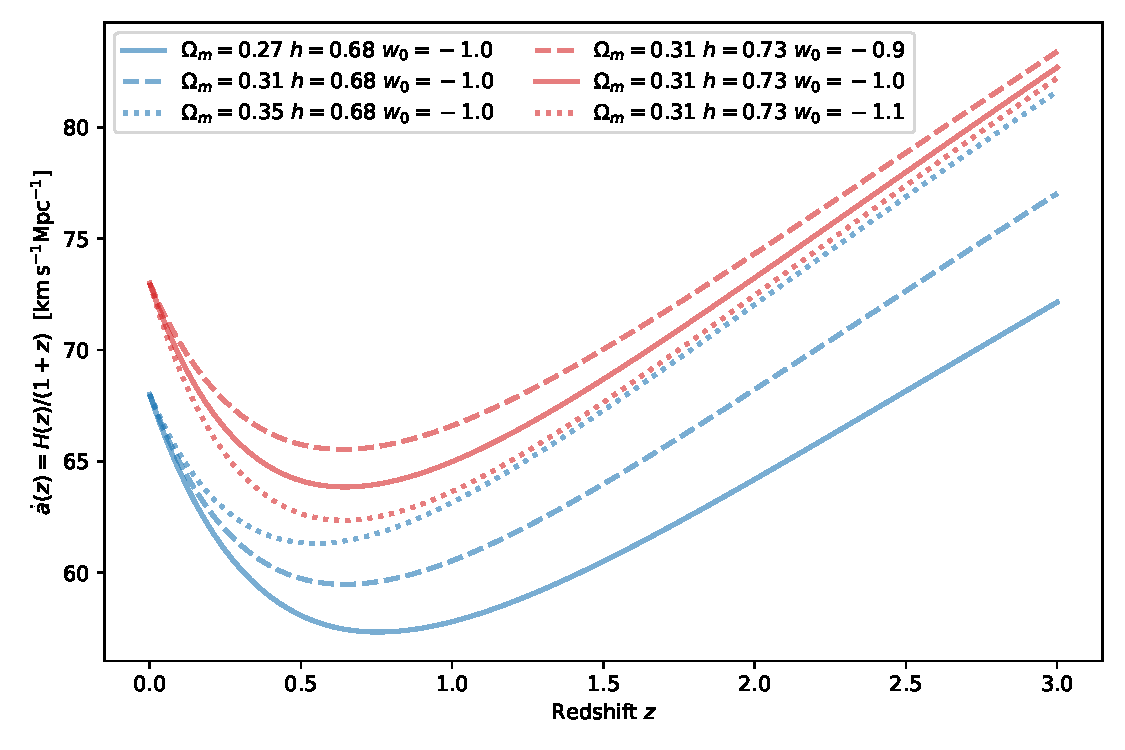
\includegraphics[width=0.9\textwidth]{fig/intro/hubble.pdf}
        \caption{The Hubble expansion rate divided by $(1+z)$, i.e., the speed of expansion $\dot{a}(z)$, 
        versus redshift $z$ for several cosmological models. }
        \label{fig:hubble_theory}
    \end{figure}

    \subsection{Distances in cosmology}
    \label{intro:model:distances}

    Distances are non-trivially defined in an expanding, potentially non-flat, Universe. 
    Therefore, different types of distances are more appropriate for certain observables.
    The \emph{Hubble distance} is related to the expansion rate as 
    \begin{equation}
        D_H(z) = \frac{c}{H(z)},
        \label{eq:hubble_distance}
    \end{equation}
    and it is commonly used in measurements of baryon acoustic oscillations in the line-of-sight 
    direction (see Chapters~\ref{chap:forests} and \ref{chap:galaxies}) or to represent the
    size of a causally connected region (in the future) of the Universe. 
    
    The \emph{comoving distance} to 
    an object at redshift $z$ is written as
    \begin{equation}
        D_C(z)  = \int_0^z \mathrm{d}z' ~ D_H(z').
        \label{eq:comoving_distance}
    \end{equation} 
    This expression yields the distance travelled by a photon from a source towards us but 
    factoring out the scale factor, effectively ``removing'' the effect of expansion. 
    
    The \emph{comoving angular diameter distance} $D_M(z)$ is useful when distances are inferred from 
    angles, which are affected by the curvature of space. 
    An object with comoving size $l$ at a redshift $z$ would be seen with an angular size $\theta$.
    This allows us to define $D_M(z) = l/\theta(z)$ as
    \begin{equation}
        D_M(z)  = D_C(z) \mathrm{sinc} \left(\sqrt{-\Omega_k} \frac{D_C(z)}{D_H(z=0)}\right),
        \label{eq:comoving_ang_diameter_distance}
    \end{equation}
    where $\mathrm{sinc}(x) = \sin(x)/x$. This distance is used in observations of 
    gravitational lensing and in measurements of the baryon acoustic oscillations 
    in the transverse direction to the line-of-sight. 
    
    Analogously, the \emph{luminosity distance} $D_L(z)$ 
    relates the flux $f$ received by an object at redshift $z$ with intrinsic luminosity $L$.
    We define then $D_L(z) = \sqrt{L/4\pi f(z)}$ as
    \begin{equation}
        D_L(z)  = D_M(z) (1+z).
        \label{eq:luminosity_distance}
    \end{equation}
    This distance is used when considering standard candles, where fluxes are used to infer 
    distances. 
    Fluxes of these standard candles vary by several orders of magnitude, 
    so it is handy to define the \emph{distance modulus} as the logarithm of the 
    luminosity distance in units of 10 parsecs (pc):
    \begin{equation}
        \mu(z) = 5\log_{10}\frac{D_L(z)}{10~\mathrm{pc}}.
        \label{eq:distance_modulus}
    \end{equation}
    This definition is such that it easily relates the observed $m(z)$ and absolute $M$ magnitude 
    of an object via $\mu(z) = m(z) - M$.

    In all distances defined above, the dependency to the cosmological energy densities
    $\Omega_x$ happens through $H(z)$ (Eq.~\ref{eq:expansion_rate}). 
    Distance measurements allow us to constrain these parameters. 
    However, all cosmological distance measurements are \emph{relative}, 
    which means they are defined to an arbitrary 
    normalisation\footnote{Two exceptions are parallax distances which are an absolute measurements
    based on the known distance between the Earth and the Sun and gravitational wave distances,
    which amplitudes depend on the distance and on the masses of the progenitors, though
    the masses affect the wave form as well, breaking the degeneracy.}, 
    such as the size of the standard ruler or the intrinsic luminosity of a standard candle.  
    One can ignore this normalisation and still constrain cosmological densities by 
    performing several distance measurements as a function of redshift.
    Or one can use some calibrated estimate of this normalisation, and estimate parameters 
    using a single distance measurement. 
    Note that in all the distances defined above, the dependency with $H_0$ only impacts
    this arbitrary normalisation, so it cannot be measured without assuming 
    the size of the ruler or the luminosity of the candles. 
    It is useful to factor out this dependency with $H_0$, and write distances 
    in units of $h^{-1}$Mpc (numerically equivalent to set $H_0 = 100$~km/s/Mpc). 
    These are the units used in the vast majority of analyses of the large-scale structures 
    and they will be also used throughout this manuscript. 
    
    \subsection{Dark energy models}
    \label{intro:model:dark_energy_models}

    In the Eq.~\ref{eq:expansion_rate} for the expansion rate of the Universe, 
    the dark energy density term is written as a general function of redshift.
    As mentioned before, the simplest model is to consider a cosmological constant
    $\Omega_{\mathrm{de}}(z) = \Omega_\Lambda$.  
    The cosmological constant can be thought as equivalent to a fluid with 
    negative relativistic pressure $p_\mathrm{de} = -\rho_\mathrm{de}$. 
    This model can be extended by considering a different equation of state 
    $p_\mathrm{de} = p_\mathrm{de}(\rho_\mathrm{de}) = w(z) \rho_\mathrm{de}$, 
    where $w(z)$ can be a constant or a more general function of redshift.
    The only constraint is that $w(z) < -1/3$, which is required to obtain 
    an accelerated expansion in a dark energy dominated Universe. 
    One widely known parametrisation is given by $w(a) = w_0 + w_a(1-a)$ 
    (\cite{chevallierAcceleratingUniversesScaling2001, linderExploringExpansionHistory2003}). 
    
    The literature contains a huge variety of models that attempt to be more physically motivated
    that those just presented (see \cite{weinbergObservationalProbesCosmic2013}, section 2.2 for a review). 
    Some of them suggest that maybe general relativity breaks down on large enough scales, 
    causing the expansion to accelerate. They suggest extensions or modifications to Einstein's 
    theory of general relativity, and are commonly known as \emph{modified gravity} models.   




\section{Model of the large-scale structures}
\label{intro:lss}

    The Universe is clearly not homogeneous and isotropic. 
    Matter clustered under the influence of gravity, creating the cosmic web,
    composed of clusters, filaments, empty regions. 
    The model described in the previous section only describes the Universe
    as a whole, without any inhomogeneities. If we want to describe 
    the evolution of the structures we need to consider an extension to
    the background model. 

    Observations of the large-scale structures and  
    the cosmic microwave background (CMB)
    indicate that the matter density field today is the evolution of 
    tiny density perturbations from the early Universe. 
    Temperature fluctuations in the CMB are of the order of $10^{-5}$, 
    while matter densities today can reach values several orders of magnitude 
    larger than the average density.
    The most widely accepted theory is that the CMB fluctuations,
    and today's structures, are originated
    from the inflation-grown quantum fluctuations, that evolved under the 
    influence of gravity and pressure in the hot dense plasma-like epoch of our Universe. 
    
    It is been possible to model the physics of the evolution of these tiny 
    fluctuations using \emph{linear perturbation theory}. The predictions of this 
    theory are an excellent match to observations of the CMB and to the late-time
    distribution of matter on large scales, i.e., larger than few tens of Mpc. 
    On smaller scales however, gravity becomes highly non-linear and more advanced 
    calculations are required. There are two main approaches to model non-linearities:
    theoretical calculations going beyond linear terms in perturbation theory 
    or numerical n-body simulations. 

    The main idea of perturbation theory is to consider that
    the density of a given species $x$ is given by:
    \begin{equation}
        \rho_x(\vec{x}, t) = \bar{\rho}_x(t)\left[1 + \delta_x(\vec{x}, t)\right],
    \end{equation}
    where the bar indicates average over the whole Universe and 
    $\delta_x \ll 1$ is a small perturbation. The average density 
    $\bar{\rho}_x$ follows the background evolution described in 
    section~\ref{intro:model}. 
    A new set of equations can be derived for the evolution of $\delta_x$ for each species 
    depending if $x$ denotes relativistic species (photons, hot baryons, hot neutrinos) 
    or non-relativistic species (cold baryons, cold neutrinos or dark matter). 
    Only some families of models also consider fluctuations in the dark energy density,
    but most commonly dark energy only acts in the background expansion. 

    The evolution of $\delta_x$ for a given species is dictated by both 
    Boltzmann and Einstein's GR equations. Boltzmann equations describe 
    the evolution of phase-space distributions of each constituent, considering
    collisions (pressure) and particle creation and annihilation. GR equations
    describe how each species influence gravitational potentials which in turn 
    make perturbations grow.

    Another important ingredient in these equations is the 
    \emph{peculiar velocities} $\vec{v}_x(\vec{x}, t)$ of 
    each species, particularly the non-relativistic ones since 
    relativistic species are assumed to have $v \sim c$. 
    Peculiar velocities directly impact the evolution of perturbations through 
    Boltzmann, Euler and continuity equations. 
    These velocities can be measured from galaxies if their distances are estimated.
    They are an important probe of the cosmological model and on the strength of 
    gravity itself. 
    They will be a key actor in chapters~\ref{chap:galaxies} and \ref{chap:velocities},
    where I will discuss redshift-space distortions and the clustering of velocities.  
    
    \subsection{Statistical description of perturbations}
    \label{intro:lss:statistics}

    The value of the matter density field at a given position $\vec{x}$ is 
    hardly observable since most of it is in the form of dark matter. 
    Only baryons which emit photons are observable. 
    Furthermore, it is impossible to learn about the physics of a single value of $\delta_m(\vec{x})$
    since we do not have access to its time evolution: our sky seems static on time-scales 
    of cosmological evolution. 
    
    In order to connect our physical model of structure growth to the observed density field,
    we turn our interest to its statistical properties. We believe that density perturbations 
    are the evolved form of quantum initial perturbations, which would follow Gaussian statistics. 
    If Gaussian, all the information of initial perturbations would be contained in its first two moments.
    The evolution of these perturbations through time modifies these initial statistical properties,
    which become highly complex, for instance creating non-Gaussianities. 
    Therefore, the final density field is described by all higher order moments as well.  

    If we focus on the density field on large scales, most of its cosmological information is
    still contained in the first moments, starting from the
    two-point function (the one-point function is zero by definition),
    which is defined as
    \begin{equation}
        \xi(\vec{x}, \vec{y}) = \langle \delta(\vec{x}) \delta(\vec{y})\rangle 
        \label{eq:two_point_function_config_space}
    \end{equation}
    where $\langle \cdot \rangle$ denotes an ensemble average. Given that
    we only have one single realisation of the Universe, we assume that
    averages over space (in an infinite space) are equivalent to ensemble averages.

    The assumptions of homogeneity and isotropy of the background can be 
    applied in an statistical sense to the perturbations. Statistical 
    homogeneity makes $\xi$ not to depend on the specific locations $\vec{x}$
    and $\vec{y}$ but only on their separation $\vec{r} = \vec{y}-\vec{x}$. 
    Statistical isotropic makes $\xi$ no longer depend on the orientation of
    $\vec{r}$, only on its absolute value $r = |\vec{r}|$. 
    Therefore, the two-point correlation function simplifies to a function of $r$:
    \begin{equation}
        \xi(r) = \langle \delta(\vec{x}) \delta(\vec{x}+\vec{r})\rangle. 
        \label{eq:two_point_function_config_space_iso_homo}
    \end{equation}
    
    The correlation function $\xi(r)$ is a powerful observable which can 
    be compared to predictions from a given cosmological model. 
    Most of my work was dedicated to measuring correlations with galaxy survey data. 

    
    \subsection{Configuration and Fourier space}
    \label{intro:lss:config_fourier}

    The time evolution of linear density perturbations $\delta(\vec{x})$ 
    is dictated by a set of second-order differential equations, containing 
    derivatives with respect to time and space. 
    It is thus convenient to apply Fourier
    transforms to these equations, where derivatives with respect to space 
    become simple products. Separations $\vec{r}$ in the so-called 
    \emph{Configuration space} become wavevectors $\vec{k}$ in 
    \emph{Fourier space}. The density perturbations in Fourier space are
    defined by 
    \begin{equation}
        \tilde{\delta}(\vec{k}) = \int \mathrm{d}^3x \ \mathrm{e}^{- i \vec{k}\cdot\vec{x}} \delta(\vec{x}),
    \end{equation}
    and its inverse is
    \begin{equation}
        \delta(\vec{x}) = \frac{1}{(2\pi)^3}\int \mathrm{d}^3k \ \mathrm{e}^{+i \vec{k}\cdot\vec{x}} \tilde\delta(\vec{k}),
    \end{equation}
    where integrals are assumed to be performed over an infinite volume. 

    As previously, we are interested in the two (or more) point functions of the
    field. In Fourier space, the two-point correlation function is known as the
    \emph{power spectrum} and is defined as
    \begin{equation}
        \left\langle \tilde\delta(\vec{k}) \tilde\delta(\vec{k})' \right\rangle = (2\pi)^3 P(k) \delta^3_\mathrm{Dirac}(\vec{k}-\vec{k}'),
        \label{eq:power_spectrum_definition}
    \end{equation}
    where $\delta^3_\mathrm{Dirac}(\vec{x})$ is a three-dimensional Dirac distribution.
    The assumption of spatial homogeneity is guaranteed by the properties of Fourier space,
    while the assumption of isotropy makes the power spectrum to be only a function of the
    absolute value of the wavevector $k = |\vec{k}|$. 

    When considering the evolution of perturbations in Fourier space to the linear level,
    each mode $\tilde\delta(\vec{k})$ evolves independently of the others. We often say 
    that there is no \emph{mode coupling} in linear theory. 

    The power spectrum $P(k)$ is an observable, as powerful as the correlation function,
    to constrain cosmological models. While in theory these two contain exactly the
    same compressed statistical information, in practice the analyses of real data  
    use different finite ranges of scales which are affected differently by systematic effects. 
    Therefore, analyses of real data in configuration and Fourier space complement each other. 
    My contributions to such analyses are presented in chapter~\ref{chap:galaxies}. 

    \subsection{Cosmological dependency of the power spectrum}
    \label{intro:lss:cosmology_dependency}

    The power spectrum $P(k)$ or the correlation function $\xi(r)$ of density 
    perturbations are excellent probes of the cosmological model. 
    They encode information accumulated over the whole Universe's history, 
    since the Big Bang until today.

    At the end of inflation, we think that perturbations were roughly Gaussian 
    (as are quantum fluctuations of the vacuum), 
    having a nearly scale independent power spectrum defined by
    \begin{equation}
        P_0(k) = A_s k^{n_s-1},
        \label{eq:initial_power_spectrum}
    \end{equation}
    where $A_s \sim 2 \times 10^{-9}$ is the amplitude of scalar perturbations 
    and $n_s \sim 0.96$ is the scalar spectral index. The term scalar refers to 
    standard density (or gravitational potential) perturbations, 
    while tensorial perturbations (of the space-time metric) refer to 
    primordial gravitational waves. Vectorial perturbations decay and rapidly become
    negligible in most common cosmological models. 

    After inflation, the majority of the energetic budget of Universe was held
    by relativistic species: photons and neutrinos. Since their energy density decays as $a^{-4}$, 
    their contribution quickly drops. This radiation-dominated era lasted until 
    $z \sim 5000$, or $t \sim 20$~kyr, when the energy density of matter became 
    the dominant source. Matter density decays at a slower rate, proportional to $a^{-3}$.
    dark energy became dominant at $z \sim 0.5$, or $t \sim 9$~Gyr, since its 
    energy density is constant (or close to constant).  
    The actual duration of each era depends on relative values of 
    the energy densities, parametrised by $\Omega_x$ 
    (see \ref{intro:model:expansion_rate}). 

    Matter perturbations grew at different rates during these different eras.
    Figure~\ref{fig:pk_evolution} shows how the power spectrum grows over time 
    for different species and for different scales. 
    In radiation-dominated era, large-scale modes (large values of $r$ 
    or small values of $k$) grew while small-scale ones oscillated,
    due to battle between gravity and radiative pressure. 
    These are known as \emph{baryon acoustic oscillations}. These oscillations
    are imprinted in the power spectrum of the photon-baryon fluid, at the time of the CMB, 
    and in the matter power spectrum at later times. 
    The radiative pressure prohibited the growth of small-scale perturbations,
    so the matter power spectrum is damped, which results in this hill-like shape. 
    In the matter-dominated era, the radiative pressure becomes negligible 
    and all modes grow equally (neglecting non-linear growth). 
    When dark energy is dominant, the expansion accelerates and 
    growth of structures slows down slightly. 
    
    \begin{figure}[t]
        \centering
        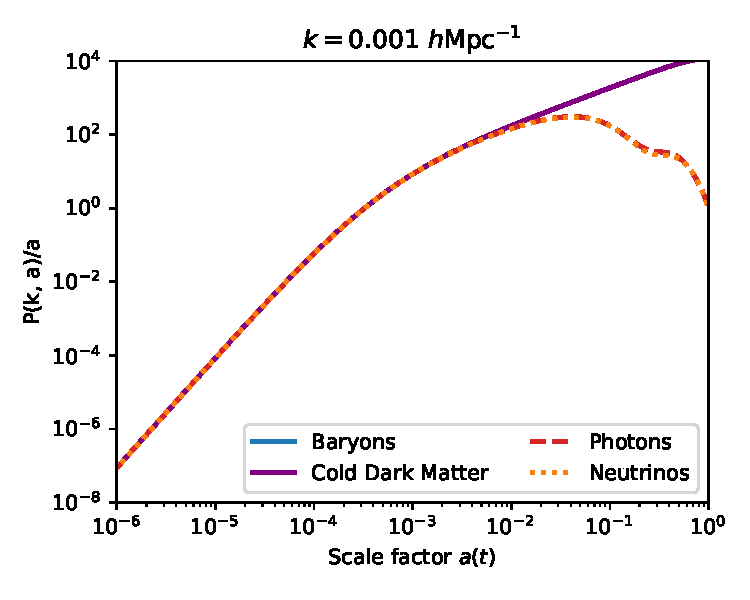
\includegraphics[width=0.49\textwidth]{fig/intro/pk_versus_time_k0.001.pdf}
        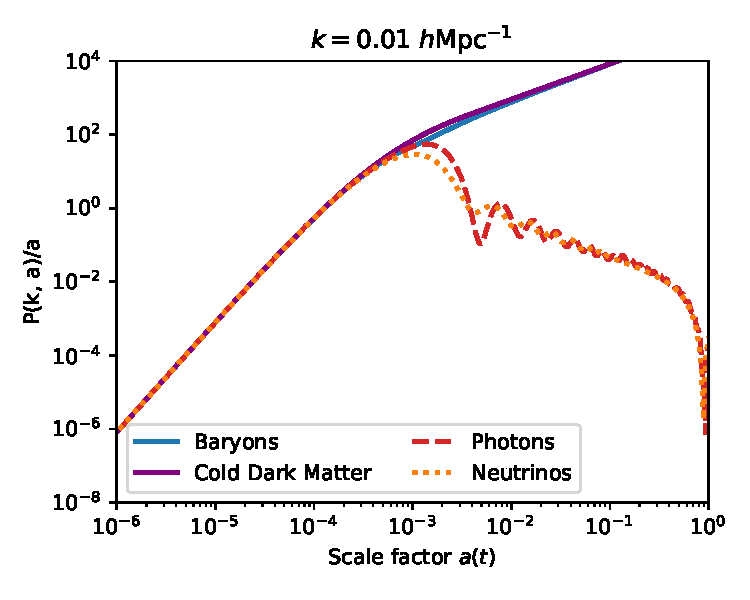
\includegraphics[width=0.49\textwidth]{fig/intro/pk_versus_time_k0.01.pdf}
        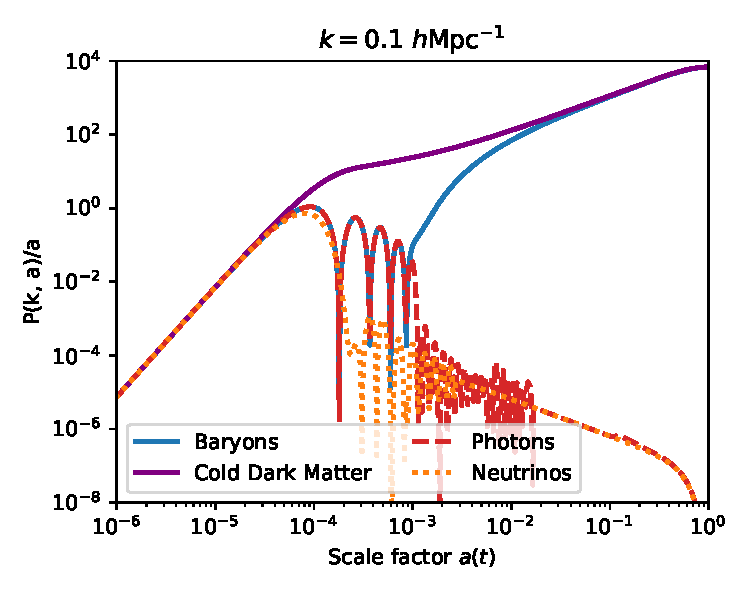
\includegraphics[width=0.49\textwidth]{fig/intro/pk_versus_time_k0.1.pdf}
        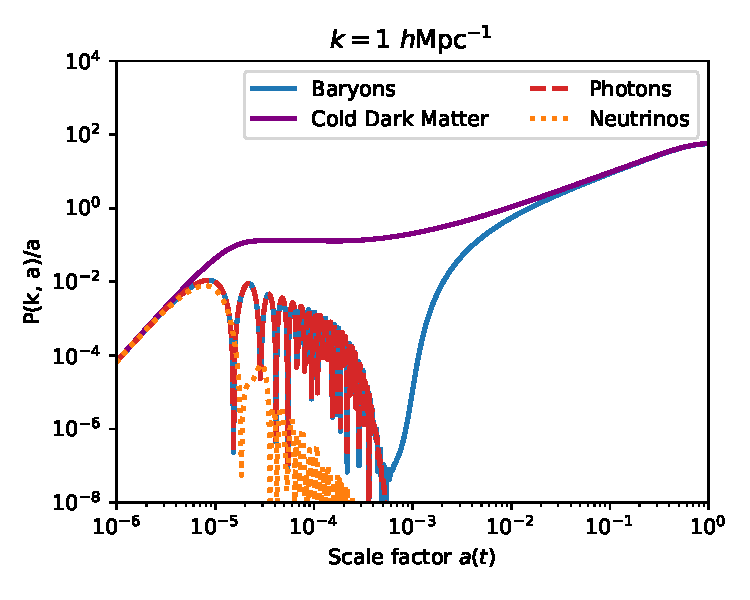
\includegraphics[width=0.49\textwidth]{fig/intro/pk_versus_time_k1.pdf}
        \caption{Evolution of the amplitude of the power spectrum versus the scale factor 
        for four different species and four different scales (one per panel). 
        The evolution was computed using \textsc{CAMB}. A movie version can be found 
        at \url{https://github.com/julianbautista/movie_correlations}.}
        \label{fig:pk_evolution}
    \end{figure}

    Well after recombination,
    matter (baryons + dark) density perturbations obey the following differential equation, if we 
    assume GR and linear theory:
    \begin{equation}
        \ddot\delta(\vec{x}, t) + 2H(z)\dot\delta(\vec{x}, t) - \frac{3}{2} \Omega_m H_0^2 (1+z)^3 \delta(\vec{x}, t) = 0. 
        \label{eq:growth_equation}
    \end{equation}

    If we assume that $\delta(\vec{x}, t) = \delta(\vec{x}, t_0) G(t)/G(t_0)$, we can factor out 
    the spatial dependency and only solve for the time-dependent term $G(t)$, known as the 
    \emph{growth factor}. Its logarithmic derivative with respect to the scale factor $a(t)$ 
    is called \emph{growth rate} of structures:
    \begin{equation}
        f(a) \equiv \frac{ \mathrm{d}~ \ln G(a)}{\mathrm{d}~ \ln a},
        \label{eq:growth_rate}
    \end{equation}
    which is a key observable for which the predicted value 
    depends on the cosmological parameters and on the assumed
    theory of gravity (e.g., GR in Eq.~\ref{eq:growth_equation}). 

    In linear theory, the peculiar velocity field is simply related to 
    density perturbations via the continuity equation 
    \begin{equation}
        \nabla \cdot \vec{v}(\vec{x}, a) 
            \equiv \theta(\vec{x}, a) 
            = -a^2 H(a) \frac{\mathrm{d}\delta(\vec{x}, a)}{\mathrm{d}a} 
            = -a H(a) f(a) \delta(\vec{x}, a) 
        \label{eq:velocity_from_density}
    \end{equation}
    where $\theta$ is the velocity divergence, a convenient scalar field describing velocities. 
    In Fourier space, the velocity field is simply proportional to the density. 
    The velocity divergence power spectrum $P_{\theta \theta}$ is an important ingredient 
    for models of redshift-space distortions, as we discuss in the following section. 

    \subsection{The amplitude of the power spectrum}
    \label{intro:lss:amplitude_power_spectrum} 
    
    The matter power spectrum $P(k)$ represents the variance of density perturbations 
    at a given wavenumber $k$. The total variance of the density field is therefore 
    the sum of all contributions over all available three dimensional modes. 
    This is equivalent to the correlation function at zero separation:
    \begin{equation}
        \sigma^2 = \xi(r=0) = \frac{1}{(2\pi)^3}\int \mathrm{d}^3k ~ P(k) = \frac{1}{2\pi^2} \int_0^\infty \mathrm{d}k ~k^2 P(k), 
        \label{eq:variance_linear_field}
    \end{equation} 
    which diverges if we use the linear prediction for the matter power spectrum.
    This is because the linear power spectrum is the evolution of a nearly scale 
    invariant power spectrum, equivalent to white noise, so the variance simply 
    keeps increasing as we consider larger ranges of scales. Therefore, it is 
    convenient to smooth the linear density field using a three-dimensional 
    top-hat filter with radius $R$. The variance of the smoothed field is 
    then 
    \begin{equation}
        \sigma_R^2 = \frac{1}{2\pi^2} \int_0^\infty \mathrm{d}k ~k^2 P(k) W_R^2(k),
        \label{eq:variance_linear_field_smoothed}
    \end{equation}
    where $W_R(k) = 3[\sin(kR) - kR \cos(kR)]/(kR)^3$ is the Fourier transform of the
    top-hat filter in three dimensions. 

    In studies of large-scales structures, it is common to use $\sigma_R^2$ 
    as a parameter defining the amplitude of the linear power spectrum. 
    As discussed before, this amplitude depends on the values of $A_s$ (Eq.~\ref{eq:initial_power_spectrum})
    and $h$, which determines the age of the Universe and how long structures could have grown.
    Therefore $\sigma_R^2$ is degenerate with $A_s$ and $h$ though is more representative of
    the amplitude of $P(k)$ at later times.  
    Other energy density parameters $\Omega_x$ also affect this amplitude, but these
    also change the overall shape and are not degenerate with $\sigma_R$. 

    The variance $\sigma_R$ is a decreasing function of $R$. Historically, 
    the chosen values for $R$ yield variances near unity, which correspond to 
    the regime where linear theory should break.   
    Recently, the value of $R = 8h^{-1}$Mpc has been used in several analysis, 
    though it has been argued that choosing $R = 12$~Mpc (without the $h$ dependency)
    is a better choice to break degeneracies (\cite{sanchezArgumentsUsingMpc2020}).
    The accepted value for $\sigma_8$ is around 0.8. 

    In measurements of redshift-space distortions and peculiar velocities, 
    there is a degeneracy between the value of $f$ and the
    amplitude of the power spectrum, $\sigma_8$. Therefore, 
    measurements can only constrain the combination $f\sigma_8$
    (see more in chapter~\ref{chap:galaxies}).


    

\section{Cosmological probes of expansion}
\label{intro:probes}

    In this section, I present the basics of the cosmological 
    observables that allow us to learn about dark energy. 
    Some of these are mostly sensitive to the background evolution
    presented in section~\ref{intro:model:expansion_rate}, while others 
    depend on the matter perturbations and their statistical properties as 
    discussed in section~\ref{intro:lss}. 

    \subsection{Direct measurements of \texorpdfstring{$H_0$}{the Hubble constant}}
    \label{intro:probes:h0}

    The Hubble constant $H_0$ is probably one of the first cosmological parameters 
    to be estimated by the person giving its name to it (\cite{hubbleRelationDistanceRadial1929}).
    Today, there are a few techniques to estimate $H_0$ which yield roughly independent results.
    See \cite{riessExpansionUniverseFaster2020} for a quick review of the latest results.  

    The most traditional method is known as the \emph{distance ladder}. 
    The idea is to measure the distance-redshift relationship of objects 
    well in the Hubble flow, i.e., far enough so they feeling the expansion. 
    The distance to the closest objects in the Solar neighbourhood can 
    be estimated with the parallax method. The Gaia satellite has the current largest catalogue 
    of parallax measurements, containing more than a billion stars. 
    Parallax is one of the few direct distance estimating methods. They can be used to 
    measure the intrinsic luminosity of some objects thought to be standard candles, such as 
    Cepheid stars, RR Lyrae, and the largest red giant stars. 
    One can use these candles to estimate distances to even more distant objects, 
    explaining the usage of the word \emph{ladder}. 
    \cite{riessCosmicDistancesCalibrated2021a} contains the latest measurements using 
    Gaia parallaxes, Cepheids and type-Ia supernovae 
    to determine $H_0 = 73.0 \pm 1.4$~km/s/Mpc.  
    \cite{freedmanCarnegieChicagoHubbleProgram2019}
    is latest measurement of distances using the tip of the red giant branch. 
    
    The distance to the galaxy NGC 4258 could be determined thanks to the presence of a 
    water maser orbiting the center of this galaxy. The proper motions of several
    clouds orbiting close to the central massive black hole could be measured both 
    in radial and angular directions, strongly constraining the dynamics of the system
    (\cite{herrnsteinGeometricDistanceGalaxy1999b}).
    The most recent measurement yields $D = 7.576\pm0.082$~(stat.)~$\pm0.076$~(sys.)~Mpc
    (\cite{reidImprovedDistanceNGC2019}), which can be used as an alternative
    to Cepheids to anchor the 
    distance ladder and provide an estimate to $H_0$. 


    Another alternative method is based on the time-delay of the signals emitted from 
    a quasar behind a strong gravitational lens. The lens creates multiple images of the
    same background quasar, but the light paths have slightly different lengths. 
    Since quasars are variable objects, the same variability is observed with a delay of 
    several days between the different images. 
    By modelling the distribution of matter between the quasar and us, 
    it is possible to convert these time delays into an estimate of $H_0$.
    The collaboration named ``$H_0$ Lenses in COSMOGRAIL's Wellspring'', or \textsc{H0LiCOW}, 
    produced the latest comprehensive measurement of $H_0$ using strongly-lensed quasars
    (\cite{wongH0LiCOWXIIICent2019}). 
    An alternative measurement has been performed using strong lenses from the Sloan (SLACS). 
    They are compared to \textsc{H0LiCOW} in \cite{birrerTDCOSMOIVHierarchical2020}. 
    
    More recently, gravitational waves from a merger of two black holes were 
    observed for the first time by the LIGO collaboration
    (\cite{theligoscientificcollaborationObservationGravitationalWaves2016}). 
    Not long after, a merger of two neutron stars was observed by both LIGO and Virgo,
    but this time an electromagnetic counterpart was also detected
    (\cite{theligoscientificcollaborationGW170817ObservationGravitational2017}), 
    pointing to the galaxy where the event occurred. Given the well predicted 
    shape of the wave form and its dependency on the masses of the neutron stars,
    it was possible to estimate the luminosity distance to the host galaxy independently of its redshift. 
    By combining this distance with an actual measurement of the host galaxy redshift, 
    a single event could provide a rough estimate of $H_0$ 
    (\cite{abbottGravitationalwaveStandardSiren2017b}). 
    This measurement opened the field of cosmology using standard sirens, i.e., gravitational wave sources. 

    The cosmic microwave background can yield an estimate of 
    $H_0$ but it is strongly degenerate with other unknown parameters, such as curvature
    or dark energy densities. Some of these degeneracies are reduced when considering 
    the effect of gravitational lensing of the CMB or when combining with other probes
    of late times. Therefore, precise measurements of $H_0$ from the CMB alone are only 
    possible when considering more restrictive models, such as a flat 
    space with a cosmological constant. 

    \subsection{Type-Ia supernovae}
    \label{intro:probes:snia}

    As mentioned earlier, type-Ia supernovae (SNIa) can be used as standard candles for 
    absolute distance measurements, if they are anchored by another method. 
    The SNIa can also be used without anchors to produce relative distance measurements and 
    constrain dark energy. In this case, the only assumption is
    that the SNIa intrinsic brightness does not evolve with redshift. 
     
    The main observable are the fluxes of SNIa as a function of time in different 
    photometric bands, known as light-curves. Spectroscopic follow up observations of 
    the explosion can confirm the type of the supernova based on the features
    present in their spectra. Another key ingredient is the redshift of the host 
    galaxy of the SNIa, which is commonly measured with spectroscopy as well.
    
    Spectro-photometric models of SNIa are used to fit the observed 
    light-curves, yielding their apparent magnitudes 
    at peak luminosity in a given photometric band. 
    These models account for correlations between colour and duration of light curves 
    and the peak magnitude, reducing the intrinsic scatter in these magnitudes from 
    40\% to roughly 15\%. 
    It is essential to obtain accurate and precise measurements 
    of SNIa fluxes in order to obtain the best cosmological constraints. 
    Large sets of realistic simulations of the data are required in order to 
    correct for selection effects. The final product of the analysis is a set
    of distance moduli (Eq.~\ref{eq:distance_modulus}) and their host-galaxy redshift, 
    which can then be compared to models of expansion of the Universe. 
    
    Distance moduli depend on dark energy through the integral of $H^{-1}(z)$ 
    (Eq.~\ref{eq:luminosity_distance} and \ref{eq:distance_modulus}). 
    In order to obtain good constraints on dark energy properties, it is 
    important to have a large redshift coverage, at least covering the 
    transition between matter-dominated to dark energy-dominated eras, so over 
    $0< z< 1$. The advantage of SNIa for dark energy studies is that they 
    can span these redshifts with a high sampling rate, which helps in 
    the study of the expansion rate. One of the inconveniences is that SNIa 
    are complex and poorly understood astrophysical events, the intrinsic 
    scatter in luminosity cannot be reduced to better than 12\%, potentially 
    limiting the gains constraining power from future experiments. 
     
    The latest comprehensive study of SNIa combines data from more than a dozen 
    projects into a single sample, the Pantheon sample, from which dark energy 
    constraints were derived (\cite{scolnicCompleteLightcurveSample2018}).
    The Dark Energy Survey also measured a more recent sample of few hundreds of SNe
    (\cite{broutFirstCosmologyResults2019a, broutFirstCosmologyResults2019, 
    kesslerFirstCosmologyResults2019}), 
    but not all  have spectroscopic classification. 
    Their constraints on dark energy are not yet competitive compared to the Pantheon sample. 
    The Zwicky Transient Facility (ZTF, \cite{grahamZwickyTransientFacility2019}) 
    is currently observing the Northern sky 
    on a search for transient events and is expected to discover around 5000 
    spectroscopically confirmed SNIa at low redshifts ($0< z< 0.12$) until 2023. 
    After 2023, the Rubin Observatory Legacy Survey of Space and Time (LSST) 
    will take over in the Southern hemisphere
    and will discover more than 300 thousand SNIa up to $z< 0.5$. 
    
    While ZTF and Rubin's samples of SNIa will not decrease significantly the 
    errors on dark energy parameters, they cover a redshift range where other 
    powerful probes, such as baryon acoustic oscillations or weak-lensing, 
    lack of statistical power due to limited volume. 
    Furthermore, at lower redshifts when dark energy is dominant, SNIa are 
    complementary to redshift-space distortions (RSD) when it comes to testing 
    the validity of GR or constraining alternative models of gravity,
    as solutions for dark energy. 

    Not only SNIa are a great probe of the 
    expansion history, they can also provide peculiar velocities of their 
    host galaxies via their inferred distances. 
    These peculiar velocities and their statistical properties can complement 
    RSD analysis when measuring the growth-rate of structures 
    (Eq.~\ref{eq:growth_rate}). Estimates of $H(z)$ and $f(z)$ can help 
    break degeneracies between simple dark energy models and more involved 
    models of gravity (\cite{kimComplementarityPeculiarVelocity2020, 
    grazianiPeculiarVelocityCosmology2020}). 
    Chapter~\ref{chap:velocities} is dedicated to this 
    topic, to which I plan to dedicate the next few years of my research.  


    \subsection{Big Bang nucleosynthesis}
    \label{intro:probes:bbn}

    In the post-inflation Universe, when temperatures
    are below the equivalent of 100 MeV, perturbations in the
    matter and radiation fields are quite 
    small and most of the physics is dictated by the interactions 
    between protons, electrons, neutrons, and photons,
    as described by the Boltzmann equations. 
    As the Universe cools down and rarefies, protons and neutrons 
    start forming atoms of deuterium, tritium, helium and heavier elements.
    This process is known as the Big Bang nucleosynthesis (BBN).

    The relative amount of each of the formed elements depends on the expansion rate 
    of the Universe at that time as well as the physical density of baryons 
    $\omega_b = \Omega_b h^2$ and radiation $\omega_r = \Omega_r h^2$.
    Given that the energies involved are within reach of particle 
    accelerators, these reactions can be studied with great detail on Earth,
    allowing us to build accurate models of the BBN 
    (see \cite{pitrouNewTensionCosmological2021} for the latest calculations
    and references therein). 
    
    Observations of the primordial abundances can be compared to the predictions 
    by BBN models. Abundances of deuterium, helium, and others can be estimated 
    from spectroscopic observations of HII regions in metal-poor galaxies 
    or from absorption lines of the intergalactic medium in quasar spectra. 
    The most up-to-date measurements of the primordial helium-4 abundance yields 
    $Y_p = 0.2453 \pm 0.0034$ (\cite{averImprovingHeliumAbundance2021}), while
    the deuterium one is $\mathrm{D/H} = (2.527 \pm 0.030) \times 10^{-5}$
    (\cite{pitrouNewTensionCosmological2021}). 
    While observations are consistent with BBN models for deuterium and helium, 
    the abundance of lithum-7 exhibits a factor 3 discrepancy, which is a huge problem 
    in BBN but quite often neglected. 
    
    The temperature fluctuations in the cosmic microwave background (CMB) are
    also very sensitive to the physical baryon density $\omega_b$. 
    Historically, the values obtained from CMB have been in good agreement 
    with BBN measurements, showing that baryons make up to around 16\% of the total 
    matter content of the Universe, or $\omega_b = (2.195 \pm  0.022)\times 10^{-2}$. 
    The agreement between two quite independent probes is one of the great successes 
    of the current cosmological model, thought they also enforce the need for a dark matter 
    component.  

   
    \subsection{Baryon acoustic oscillations}
    \label{intro:probes:bao}

    Baryon acoustic oscillations (BAO) is the name given to the propagation of sound
    waves in the primordial plasma (baryons and photons), prior to recombination. 
    Because of the high pressure on small scales at those times, 
    each initial density perturbation had a spherical density wave around them 
    propagating outwards at the speed of sound in that medium. The speed of sound
    in the plasma is given by 
    \begin{equation}
        c_s(z) \equiv \sqrt{\frac{1}{3[1+R(z)]}}
        \label{eq:sound_speed}
    \end{equation}
    where $R(z) = 3\rho_b / 4 \rho_\gamma$ is the baryon-to-photon ratio.
    The propagation of sound waves occurred until the temperatures and densities 
    dropped to values such that baryons no longer 
    felt the pressure from photons, known as the \emph{drag epoch}, which is 
    close in time to the recombination (but technically not the same epoch), at $z\sim 1100$. 
    This process left a slight over dense shell of matter around each initial perturbation
    with a radius given by 
    \begin{equation}
        r_\mathrm{drag} \equiv r_s(z_\mathrm{drag}) = 
            \int_\infty^{z_\mathrm{drag}} \mathrm{d}z' \frac{c_s(z')}{H(z')}
        \label{eq:sound_horizon}
    \end{equation}
    which is known as the \emph{sound horizon at drag epoch}, or the BAO scale. 
    Today, $r_d$ has a physical size of about 147 Mpc, much larger than any 
    collapsed structure in the Universe. 
    As one can see from Eqs.~\ref{eq:sound_speed}
    and \ref{eq:sound_horizon}, $r_\mathrm{drag}$ mainly depends on 
    $\omega_b$ and $\omega_c$ assuming the CMB gives a precise 
    estimate of $\omega_\gamma$. The dependency of $r_\mathrm{drag}$ 
    is mainly through $\omega_b$.

    After recombination, the sound horizon scale only increases in size 
    due to the expansion, or equivalently, its comoving size remains unchanged. 
    Therefore, the BAO scale is a great \emph{standard ruler} to study the expansion 
    rate of the Universe. 
    In practice, the BAO scale is observed statistically in the 
    two-point function of the matter density field, so it is often 
    classified as an statistical standard ruler. 
    In configuration space, the correlation function $\xi(r)$ presents a small 
    peak at separations corresponding to the BAO scale $r_d$, while in Fourier space 
    the power spectrum $P(k)$ contains an oscillatory pattern as a function of scale 
    with a period proportional to the BAO scale.  
    In chapters~\ref{chap:forests} and \ref{chap:galaxies}, I present 
    my past work in the measurement of the BAO scale using \lya\ forests 
    and galaxies, respectively, as tracers of the matter density field.
    
    Given that a galaxy survey is made of angular positions and redshifts, 
    which are true observables, 
    the BAO peak is effectively measured as an angle $\Delta \theta_\mathrm{BAO}$ 
    or as a difference in redshift $\Delta z_\mathrm{BAO}$. 
    These can be modelled as ratios of distances to the BAO scale $r_d$ as
    \begin{equation}
        \Delta \theta_\mathrm{BAO}(z_\mathrm{eff}) = \frac{D_M(z_\mathrm{eff})}{r_d}
        \label{eq:bao_angular}
    \end{equation}
    \begin{equation}
        \Delta z_\mathrm{BAO}(z_\mathrm{eff}) = \frac{D_H(z_\mathrm{eff})}{r_d}
        \label{eq:bao_radial}
    \end{equation}
    where $z_\mathrm{eff}$ is the effective redshift of the galaxy survey, 
    $D_M$ is the comoving angular diameter distance (Eq.~\ref{eq:comoving_ang_diameter_distance}),
    and $D_H$ is the Hubble distance (Eq.~\ref{eq:hubble_distance}). 

    There are two ways BAO can be used to constrain cosmological models, 
    depending if we assume that $r_\mathrm{drag}$ is known or not. 
    If $r_\mathrm{drag}$ is known, i.e. given by Eq.~\ref{eq:sound_horizon} 
    using some value for $\omega_b$
    (given by the CMB or BBN for instance), then BAO measurements
    are converted to absolute distance measurements which depend only on  
    $H(z)$. Therefore, BAO can constrain $H_0$, curvature and dark energy. 
    If $r_\mathrm{drag}$ is supposed to be unknown but still a standard ruler, 
    then BAO constraints the ratio of $E(z) = H(z)/H_0$ to the combination 
    $H_0 r_\mathrm{drag}$ which is now degenerate. This is similar to the case of
    type Ia supernovae, where their absolute magnitude is degenerate with $H_0$.
    By combining several BAO measurements at different effective redshifts, 
    BAO is a powerful probe of dark energy and curvature. 

    Current BAO measurements span effective redshifts from 0.1 to 2.3.
    The Sloan Digital Sky Survey (SDSS, 
    \cite{eisensteinSDSSIIIMassiveSpectroscopic2011, blantonSloanDigitalSky2017}) 
    has measured more than 2 million 
    redshifts spectroscopically in the past twenty years, 
    producing the largest maps to date of the
    distribution of matter in the Universe. In addition to SDSS, 
    surveys such as FastSound (\cite{okumuraSubaruFMOSGalaxy2016}), 
    Vipers (\cite{pezzottaVIMOSPublicExtragalactic2017}),
    6 degree field galaxy survey (6dFGS, \cite{beutler6dFGalaxySurvey2012a})
    and WiggleZ (\cite{parkinsonWiggleZDarkEnergy2012}) also
    produced BAO measurements using galaxies, though the volumes 
    probed and the number of galaxies is inferior to SDSS. 
    The latest cosmological constraints from BAO are described in 
    \cite{alamCompletedSDSSIVExtended2021}.



    \subsection{The cosmic microwave background}
    \label{intro:probes:cmb}

    The cosmic microwave background (CMB) is one of the richest cosmological probes of all. 
    The photons we receive today last scattered on baryons at a redshift of about 1100,
    corresponding to roughly 380 000 years after the Big Bang. 
    It is currently the oldest information that we can measure from the Universe today. 
    
    The average temperature $T_\mathrm{CMB} = 2.72548 \pm 0.00057$~K 
    (\cite{matherMeasurementCosmicMicrowave1994, fixsenTemperatureCosmicMicrowave2009}) 
    of these photons, measured by the COBE satellite, tell us on how much 
    energy density from radiation there is in the Universe. 
    Considering a black body Bose-Einstein distribution for the photons, we have that 
    \begin{equation}
        \rho_\gamma = \frac{\pi^2 k^4}{15 \hbar^3 c^3} T_\mathrm{CMB}^4
        \label{eq:energy_density_photons}
    \end{equation} 
    
    The fluctuations around this average temperature, $\Delta T$, 
    and the polarisation of these photons
    trace the structures back at the recombination epoch. 
    Given its early-times nature, 
    the temperature and polarisation fields are extremely well described by 
    Gaussian statistics. Most of the information is therefore contained in the two point
    functions of these fields. Given that these fields are functions of
    the position angle in the sky $(\theta, \phi)$, it is convenient to decompose these 
    fields into a basis of spherical harmonics $Y_{\ell m}(\theta, \phi)$.
    The amplitude of each harmonic is denoted $a_{\ell m}$. The angular power spectrum  
    is simply the variance of these amplitudes: $C_\ell = \langle a_{\ell m} a^*_{\ell m}\rangle$, 
    which in linear theory is simply a function of $\ell$ and independent of $m$. 
    The temperature and both E and B polarisation modes of the CMB can be decomposed into 
    spherical harmonics, so we can estimate all cross power spectra, e.g., 
    $C^{TE}_\ell = \langle a^T_{\ell m} a^{E*}_{\ell m}\rangle$ is the
    cross temperature and E-mode polarisation power spectrum. 
    
    The temperature and polarisation auto and cross power spectra 
    are exquisitely well modelled by linear perturbation theory. 
    In the most basic $\Lambda$CDM model, the power spectrum is a 
    function of only six parameters: the angular scale of baryon 
    acoustic oscillations $\theta_*$, 
    the physical density of baryons $\omega_b$ and dark matter $\omega_c$, 
    the primordial power spectrum amplitude $A_s$ and slope $n_s$, 
    and the optical depth to the last scattering surface $\tau$.
    The fact that such a model with so few free parameters can 
    describe so well CMB observations is one of the greatest achievements 
    in modern physics. 
    A great description of the CMB physics 
    from first principles can be found in \cite{dodelsonscottModernCosmology2nd2020}.
    Several codes are available to compute models for the CMB 
    such as \textsc{CAMB}\footnote{\url{https://camb.info/}} 
    (\cite{lewisEfficientComputationCosmic2000})
    and \textsc{CLASS}\footnote{\url{https://lesgourg.github.io/class_public/class.html}} 
    (\cite{lesgourguesCosmicLinearAnisotropy2011}). 
    
    Since COBE measurements, all experiments focus on measuring exclusively 
    anisotropies in temperature and polarisation. 
    The current reference results based on the CMB come from the Planck satellite.
    (\cite{planckcollaborationPlanck2018Results2020}). Since it is a satellite, it has
    access to the full sky and thus the very large scale modes. 
    The angular resolution of the instrument of about 5 arcmin allows 
    a precise measurement of the power spectrum up to $\ell \sim 2500$. 
    Eight acoustic peaks are observed, yielding an extremely tight constraint 
    on $\theta_*$. The relative amplitudes of the acoustic peaks is sensitive to 
    $\omega_b$ and $\omega_c$. The overall amplitude of the spectrum yields the 
    $A_s \text{e}^{-2\tau}$, while its dependency with scale yields $n_s$. 
    Polarisation spectra break the degeneracy between $A_s$ and $\tau$. 
    A weak constraint on dark energy is possible thanks to the integrated Sachs-Wolfe effect 
    at low redshift.

    On Earth, several experiments were build achieving higher angular resolution
    or a higher depth in observations. 
    Both the Atacama Cosmology Telescope (ACT, \cite{aiolaAtacamaCosmologyTelescope2020})
    and the South Pole Telescope (SPT, \cite{aylorComparisonCosmologicalParameters2017, 
    balkenholConstraintsLambdaCDM2021, 
    dutcherMeasurementsEModePolarization2021}), measured temperature and polarisation power spectra 
    on a smaller fraction of sky but reaching up to $\ell \sim 9000$.
    The BICEP/Keck (\cite{bicep/keckDemonstrationImprovedConstraints2021}) focused on 
    the polarisation signal over large angular scales (low $\ell$) with the goal of
    measuring the effect of primordial gravitational waves caused by inflation.  
    Due to strong contamination by polarised emission from Galactic dust, 
    currently there is no detection of such primordial signal. 
    New experiments will increase even further the sensitivity and the number of detectors,
    in order to achieve this goal. 




 

    \subsection{Redshift-space distortions}
    \label{intro:probes:rsd}

    Matter is not static in the Universe. 
    Due to gravity, matter flows from underdense regions towards overdense ones,
    so it can be described as a fluid following some velocity field. 
    These velocities are commonly called \emph{peculiar velocities}.
    The radial component of peculiar velocities with respect to the observer 
    alters the observed redshift of an object, due to the Doppler effect. 
    The total observed redshift $z_\mathrm{obs}$
    is a combination of its cosmological redshift $z_\mathrm{cos}$, 
    due to the expansion of the Universe,
    and the peculiar redshift $z_\mathrm{pec}$, due to the Doppler effect:
    \begin{equation}
        1 + z_\mathrm{obs} = (1 + z_\mathrm{cos})(1 + z_\mathrm{pec})
        \label{eq:observed_redshift}
    \end{equation}
    where
    \begin{equation}
        z_\mathrm{pec} = \sqrt{\frac{1 + \frac{\vec{v}\cdot \hat{n}}{c} }{1 - \frac{\vec{v}\cdot \hat{n}}{c}}} - 1
                        \approx \frac{\vec{v}\cdot \hat{n}}{c}
        \label{eq:peculiar_redshift}
    \end{equation}
    The first equality is the definition of the relativistic Doppler effect, 
    $\vec{v}$ is the velocity and $\hat{n}$ is the radial unitary vector.  
    The right-hand side is the non-relativistic approximation, which is accurate
    for typical velocities of matter flows in our Universe, of the order of few hundreds of \kms. 

    When converting observed redshifts into comoving distances, peculiar velocities
    introduce a small error such that 
    \begin{equation}
        s(z_\mathrm{obs}) \approx r(z_{\mathrm cos}) + \frac{(1+z_\mathrm{cos})}{H(z_\mathrm{cos})}\vec{v} \cdot \hat{n},
        \label{eq:redshift_space_distance}
    \end{equation}
    where $s$ is the \emph{redshift-space} distance and $r$ is the \emph{real-space} distance.
    These errors distort the observed distribution of matter/galaxies in the radial direction. 
    This effect is observable and manifests as anisotropy (radial versus transverse) 
    in the two-point functions of the density field.
    These anisotropies are named \emph{redshift-space distortions} (RSD). 
    The RSD are a powerful probe of the dynamics of the matter field, i.e., 
    how velocities are related to the densities, and how they contribute
    to the growth of structures over time. More generally, 
    observations of RSD can be used to test the validity of general 
    relativity since it is a probe of the strength of gravity. 

    The density contrast of matter is modified when observed in redshift-space relative 
    to real-space. Mass conservation implies that
    \begin{equation}
        [1+\delta_s(\vec{s})] \dinteg^3s = [1+\delta(\vec{x})]\dinteg^3 x,
        \label{eq:mass_conservation}
    \end{equation}
    such that in Fourier space we obtain, in the linear regime 
    (\cite{kaiserClusteringRealSpace1987})
    \begin{equation}
        \delta_s(\vec{k}) = (1 + f \mu^2 )\delta(\vec{k})
        \label{eq:delta_rsd_fourier}
    \end{equation}
    where $f$ is the growth-rate of structures defined in Eq.~\ref{eq:growth_rate} 
    and $\mu = \vec{k} \cdot \hat{n} / k$ is the cosine of the angle between the wavevector 
    and the line of sight. 
    The power spectrum in redshift-space assuming linear 
    perturbations is simply 
    \begin{equation}
        P_s(k, \mu) = (1 + f\mu^2)^2 P_m^\mathrm{lin}(k)
        \label{eq:power_spectrum_rsd_linear}
    \end{equation}
    
    This means that the redshift-space matter power spectrum has radial modes enhanced 
    by a factor of $(1+f)^2$ (where $f \sim 1$) relative to modes transverse to the line 
    of sight. This enhancement is observable with galaxy surveys. If the normalisation 
    of the linear matter power spectrum is parametrised by $\sigma_8$ 
    (Eq.~\ref{eq:variance_linear_field_smoothed}), then the actual measured quantity is 
    the product $f\sigma_8$. Transposed to a given effective redshift $z_\mathrm{eff}$
    of a galaxy survey, we need to scale $\sigma_8$, which is usually defined at $z=0$, 
    using the growth factor $G(z)$, such that the measured quantity is $f(z)\sigma_8 G(z)$.
    Some works use the notation $\sigma_8(z) \equiv \sigma_8 G(z)$. 
    
    The observable $f(z)\sigma_8(z)$ is mostly sensitive to the amount of 
    dark matter $\omega_m$, which drives the growth of structures, 
    and $H(z)$, which damps the growth (see Eq.~\ref{eq:growth_equation}). 
    Therefore, measurements of $f(z) \sigma_8(z)$ versus redshift can be 
    used to constrain dark energy models or alternatives to GR.

    The latest most relevant measurements were performed using data from 
    the Sloan Digital Sky Survey (SDSS), including 
    \begin{itemize} 
        \item the SDSS Main Galaxy Sample \cite{howlettClusteringSDSSMain2015},
        \item the Baryon Oscillation Spectroscopic Survey (BOSS, \cite{alamClusteringGalaxiesCompleted2017}), 
        \item the extended BOSS luminous red galaxy sample (eBOSS LRG, \cite{bautistaCompletedSDSSIVExtended2021, gil-marinCompletedSDSSIVExtended2020}), 
        \item the eBOSS emission line galaxy sample (eBOSS ELG, \cite{tamoneCompletedSDSSIVExtended2020, demattiaCompletedSDSSIVExtended2021}),
        \item the eBOSS quasar sample (eBOSS QSO, \cite{houCompletedSDSSIVExtended2021, neveuxCompletedSDSSIVExtended2020}),
    \end{itemize}

    In chapter~\ref{chap:galaxies} I present my contributions to the measurement 
    of the growth-rate of structures using the eBOSS LRG sample 
    (\cite{bautistaCompletedSDSSIVExtended2021}).
    The cosmological implications of SDSS growth-rate measurements are described 
    in \cite{alamCompletedSDSSIVExtended2021}. 

    \subsection{Weak gravitational lensing}
    \label{intro:probes:wl}

    Photons follow space-time geodesics. Space-time is distorted in the presence 
    of a source of gravitational potential, which is typically a mass concentration. 
    Therefore, the matter distribution in the Universe bends trajectories of photons 
    travelling from distant sources.  
    This phenomenon receives the name of \emph{gravitational lensing}, since the 
    theory describing light propagation on a gravitational field is analogous to classical optics.  
    Gravitational lensing is a rich cosmological probe since the distortion of photon trajectories
    depends on both the baryonic and dark matter. From lensing measurements we can learn 
    about the total matter distribution in an expanding Universe. 
    
    In the case of an extended source of photons, e.g., a galaxy, light from different 
    locations within the source take slightly different paths towards the observer. 
    If this source is placed in the background of a mass concentration - the lens - each 
    path will suffer a slightly different bending, which depends on the impact parameter 
    of each photon relative to the center of this lens. 
    Also, due to conservation of surface brightness, the total flux is also increased. 
    The final result is an image that is shifted, distorted and brighter. 

    Lensing measurements use shifts, distortions and the increase in fluxes to determine 
    properties of the lenses. These measurements are difficult since we do not have access to 
    the original unlensed positions, shapes or fluxes of source galaxies. 
    One remarkable exception is lensing in its strong regime. 
    If the impact parameter of the source relative to the centre of the lens is below some threshold, 
    the Einstein radius, multiple images of the same source are created. 
    Strong lensing allows us to estimate the mass and density profile of a given lens. 
    Moreover, if the source is variable in time, this variability is slightly delayed 
    between each of the multiple images, which allows us to constrain the expansion 
    of the Universe. As mentioned in section~\ref{intro:probes:h0}, strongly lensed 
    quasars (variable sources) are used to constrain $H_0$, under the assumption 
    that we can properly model the lens density profile. 

    In the weak lensing regime, only statistical measurements can be performed. 
    The main idea is that galaxy shapes can be approximated by ellipses which have 
    an intrinsic distribution of ellipticities and orientations. 
    The matter density field between the observer and source galaxies slightly modifies 
    these shapes and orientations. 
    These changes are observable at the two-point statistics level. 
    Two key ingredients make this measurement challenging: galaxy shapes and redshifts. 
    A weak lensing survey is a photometric survey trying to optimise the sky coverage and 
    image quality. Billions of galaxies have been detected in the state-of-the-art surveys. 
    The shapes of the galaxies are affected by the point-spread function of the images, 
    which is a combination of atmospheric and instrumental dispersion. 
    These effects have to be very well characterised and understood. 
    Galaxy shapes are then converted into shear estimates. 
    A spectroscopic measurement of the redshift for all galaxies is unfeasible with today's technology,
    so they are estimated using the fluxes measured in a few photometric bands. 
    The precision of the redshift is therefore degraded, typically of the order of $\sigma_z \sim 0.05(1+z)$, 
    but since weak lensing is mostly an angular effect, these uncertainties do not play a major role. 
    
    With a sample of billions of galaxies with their measured shapes and photometric redshifts, 
    three types of two point functions can be computed. 
    First, the angular two-point correlation function of galaxy positions $w(\theta)$ as in standard galaxy clustering. 
    Second, the cross correlation between galaxy positions and the shear of galaxies around them.
    Typically one considers positions from the lenses and the shear of background source galaxies.
    Also, one considers only the tangential component of the shear relative to each galaxy, where the signal 
    is maximal, in contrast with the radial component. We denote this cross correlation $\gamma_t(\theta)$. 
    This second statistics is also referred to as \emph{galaxy-galaxy lensing}. 
    Third, the auto correlation of shear also known as \emph{cosmic shear}. 
    The shear-shear correlations can be projected into two orientations, 
    so they actually give two statistics $\xi_{+}(\theta)$ and $\xi_{-}(\theta)$. 
    
    The model for the shear of a source galaxy is given by a sum of many layers of matter acting as thin lenses. 
    As in classical optics, the impact of each lens layer depends on the distances between observer-lens and lens-source. 
    The maximum effect is when the lens is at mid-distance between the observer and the source. 
    The model for the two-point functions is therefore an integral of the matter power spectrum, weighted by the distances
    of the lenses and sources. 
    The angular power spectra are computed and converted into configuration space.
    Given this dependency on both geometry and the amplitude of the power spectrum, 
    weak lensing measurements are sensitive to the combination defined as  
    $S_8 = \sigma_8 \sqrt{\Omega_m/0.3}$.

    The most recent measurements have been mainly carried out by three projects. 
    Similarly to the case of the CMB, one large project observed a large area of the sky 
    while two smaller projects observed a smaller patch of the sky to greater depth. 
    The Dark Energy Survey (DES) released recently their cosmological analysis of the Year 3 sample 
    \cite{descollaborationDarkEnergySurvey2021}). They measured 5000 deg$^2$ of the Southern sky 
    using a 570 Megapixel camera in five photometric bands up to a limiting magnitude of 23. 
    More than 100 million galaxies had their shapes and redshifts measured. 
    This state-of-the-art sample for weak lensing measurements obtained $S_8 = 0.776 \pm 0.017$
    and $\Omega_m = 0.339^{+0.032}_{-0.031}$
    when assuming flat $\Lambda$CDM. In a $w$CDM model with 
    varying equation of state for dark energy, they obtain 
    $S_8 = 0.775^{+0.026}_{-0.024}$, $\Omega_m = 0.352^{+0.035}_{-0.041}$ and $w_0 = -0.98^{+0.32}_{-0.20}$. 
    The Kilo Degree Survey (KiDS) measured a smaller patch of 1350 deg$^2$ of the Southern sky 
    in nine optical and infrared bands. Since they area is not as large as DES, 
    they combine their lensing measurements with clustering from the BOSS survey \cite{heymansKiDS1000CosmologyMultiprobe2021}). 
    The Subaru Hyper Supreme Cam (HSC) is a deep survey to be carried out over 1400~deg$^2$ 
    in five optical bands up to a limiting magnitude of 26. Results from the first year of data covering 137 deg$^2$ 
    can be found in  \cite{hikageCosmologyCosmicShear2019} but their constraints on $S_8$ are still quite broad
    compared to those from DES. 

    Future surveys such as Rubin-LSST and Euclid will significantly improve constraints from weak lensing. 
    Rubin-LSST will observe most of the Southern sky to similar depth as HSC, while Euclid will be 
    the first space program able to produce weak lensing measurements. The great advantage of Rubin-LSST 
    is the large number of optical and near-infrared bands while Euclid does not suffer from atmospheric effects 
    and will have the best galaxy shape measurements. 
    The synergy between these two surveys has been widely explored in the literature 
    (\cite{jainWholeGreaterSum2015, rhodesScientificSynergyLSST2017, capakEnhancingLSSTScience2019}). 
    



